\chapter{Background}
This chapter will give some background on important algorithms and file formats used in this project. It will also give an introduction to the snow simulator.

\section{Search Algorithms and A* Shortest Path Search Algorithm}
Finding the shortest path between nodes in a graph is an old and heavily researched problem. The problem can be stated like this: Given a weighted graph $G = (V,E)$ with edges $E$ and vertices $V$, and a weighting function $w(e) = w(v_i, v_j)$ of edge $e = (v_i, v_j)$, find the path from $v_a$ to $v_b$, that solves the minimization problem

\begin{equation}
\min_{\mbf P} \left\{ \sum_{e\in \mbf{p}} w(e) \right\}
\end{equation}

over all paths $\mbf P$ between nodes $v_a$ and $v_b$.

\subsection{Solving shortest path problems}
There are many algorithms to solve the minimization problem of finding the shortest path. There are two main categories: Single-source, and all-pairs. Single-source solves the shortest path algorithm for a single source node $a$, to one or all other nodes. All-pairs finds, as the name suggests, the shortest path between all the nodes in the graph. In this project, we are concerned about the single-source shortest path algorithms. In particular, we are interested in finding the shortest path between one node $v_a$ to another single node $v_b$.

\subsubsection{Dijkstra's algorithm}
One of the most well known and efficient single-source algorithms when we assume that we have no knowledge of the graph, is Dijkstra's algorithm. Dijkstra's algorithm is descriped in algorithm \ref{alg:dijkstra}. The basic idea behind the algorithm is to always choose to look at the neighbors of the node currently closest to the starting node that has not yet been explored. To retrieve the actual path, we keep a pointer to the predecessor of each node, which is updated once a better path to that node has been found. 

\begin{algorithm}
\begin{algorithmic}
\STATE Initially, set the distance to the source $d(v_a)=0$ and for all other nodes $d(v_i) = \infty$.
\STATE Let $\pi(v)$ be the predecessor to node $v$; initially, $\forall v (\pi(v) = \mbox{none})$ 
\STATE Put all nodes $v_i$ in a priority queue, sorted on $d(v_i)$.
\WHILE {$|Q| > 0$}
    \STATE $v \gets \mbox{next node in Q}$
    \STATE $Q\gets Q - \{v\}$
    \FORALL{neighbors $w$ of $v$}
        \IF{$d(v)+w(v,w) < d(w)$}
            \STATE $d(w) \gets  d(v)+w(v, w)$.
            \STATE $\pi(w)\gets v$
        \ENDIF
    \ENDFOR
\ENDWHILE
\end{algorithmic}
\caption{Pseudocode for Dijkstra's algorithm}
\label{alg:dijkstra}
\end{algorithm}

After the algorithm finishes, we have the total cost of the shortest paths from the source $v_a$ to all other nodes. The time complexity, when implemented efficiently with a fibonacci heap, is $O(|E|+|V|\log |V|)$\cite{fibodijkstra}. One useful observation is that the shortest path to the node we pick from the queue is optimal; this is due to the fact that all other nodes in the queue has a larger or equal distance from $v_a$, and thus, assuming non-negative edges, we can not hope to find a better path.. Because of this, if we are only interested in the path from $v_a$ to $v_b$, we can stop the algorithm once we pick $v_b$ from the queue. 

\subsubsection{Utilizing knowledge about graph topology: A*}
In many practical cases, we have specific knowledge about the graph topology. For instance, if we seek to find the shortest path from the city of Oslo to Trondheim, we know, for instance, that if we move in the right direction (i.e. north), we are most probably closer than we were, and we know that we need to travel AT LEAST the straight line distance from Oslo to Trondheim. This kind of knowledge can be utilized in making more efficient single-source, single-destination shortest path algorithms, by computing heuristics on the cost from each node to the goal. One such algorithm is A*.\cite{astar}

A* is an extension of Dijkstra's algorithm. We define $g(x)$ as the distance from the start node $v_a$ to node $x$ ($g(x)$ is the same as $d(x)$ in Dijkstra's algorithm, but it is common to denote this function as $g(x)$ in literature). We also define the heuristic $h(x)$ as an {\textit admissive} (optimistic) and {\textit consistent} (monotone) estimate of the cost from node $x$ to the goal node $v_b$. That the heuristic is optimistic simply means that it never over-estimates the distance left to the goal, i.e. $h(x) \leq h^*(x)$, where $h^*(x)$ is the {\textit optimal} heuristic function, that give the exact cost from node $x$ to the goal node $v_b$. That the heuristic is consistent, means that the search will never take a step back. This is described later.

Combining these values gives the {\textit f-cost} $f(x) = g(x)+h(x)$, which is the actual estimate on the distance from the start node $v_a$ to the goal node $v_b$. The algorithm is outlined in algorithm \ref{alg:astar}.

\begin{algorithm}
\begin{algorithmic}
\STATE Maintain a queue $OPEN$ and a set $CLOSED$. 
\STATE Initially, $OPEN = \{v_a\}$ and $CLOSED = \emptyset$. 
\STATE Let $\pi(v)$ be the predecessor to node $v$; initially, $\forall v (\pi(v) = \mbox{none})$ 
\WHILE {$|Q| > 0 \land v_b \notin CLOSED$}
    \STATE $v \gets \mbox{node with smallest f-cost in OPEN}$
    \STATE $OPEN\gets OPEN - {v}$
    \STATE $CLOSED \gets CLOSED + \{v\}$
    \FORALL{neighbors $w$ of $v$}
        \IF{$w \notin CLOSED \land w \notin OPEN$}
            \STATE Put $w$ in the $OPEN$ queue.
        \ELSIF{$w \in OPEN \wedge g(v)+w(v,w) < g(w)$}
            \STATE $g(w) \gets g(v)+w(v,w)$
        \ENDIF
    \ENDFOR
\ENDWHILE
\end{algorithmic}
\caption{Pseudocode for A* shortest path algorithm}
\label{alg:astar}
\end{algorithm}

The main difference from the regular Dijkstra's algorithm, is how nodes are picked from the queue. Instead of picking the node with the lowest $g(x)$ as we do with Dijkstra, we pick the node with the lowest f-cost, $f(x) = g(x) + h(x)$. This way we prefer nodes that are "closer" to the goal. As a side note, if we set $h(x)=0$, the A* algorithm is reduced to Dijkstra's algorithm. If we use the example of finding the shortest route from Oslo to Trondheim, if we use Dijkstra, nodes will be expanded in all directions, i.e. Dijkstra will search both south, west and east, which is unneccesary work. If we instead use A*, nodes south of Oslo may still have a small distance from the start, but will have a higher $h(x)$ than those to the north, and thus may not be selected for expansion. Figure \ref{fig:astar_vs_dijkstra} shows the expanded nodes for a simple shortest path problem where $w(v,w)=1$ for all pairs of neighbors $v,w$, and the neighbors are the neighboring four nodes.

\begin{figure}[ht]
\centering
\subfloat[A* expansions]{\includegraphics[width=0.40\textwidth]{figure/astar_expansion}}
\qquad
\subfloat[Dijkstra expansions]{\includegraphics[width=0.40\textwidth]{figure/dijkstra_expansion}}
\caption{Expanded nodes in A* vs. Dijkstra}
\label{fig:astar_vs_dijkstra}
\end{figure}

\subsubsection{Designing the heuristic. Admissibility and consistency}
In order to guarantee that the A* algorithm is optimal, the heuristic function $h(x)$ must be admissible and consistent\cite{astar}. That $h(x)$ is admissible means that $h(x) \leq h^*(x)$ where $h^*(x)$ is the optimal heuristic that gives the exact distance to the goal from a node $x$. More intuitively, this means that $h(x)$ is an {\textit optimistic} estimate of the cost: the estimate is at most the actual cost. For pathfinding in euclidean space, e.g. in $\mathbb{R^3}$, an admissible heuristic is the straight line distance to the goal; the actual cost to the goal may, however, be higher due to obstacles.

A consistent, also called monotonic heuristic is a heuristic that fulfills the requirement $h(x) \leq w(x,y) + h(y) \Leftrightarrow h(x)-h(y) \leq w(x,y)$. This means that we will never take a step back, because the cost of getting to $y$ from $x$ is greater (or equal to) the difference in the estimates. This implies that if $x$ is the node being explored, we can never find a better $g(x)$ by going through $y$ from $x$; we will always have a monotonically increasing total cost for the best path, as the search goes on. The straight line distance in euclidean space $\mathbb{R^n}$ is a consistent heuristic for the shortest path between two points, because moving in any direction will give a greater or equal total f-cost for the path. It is equal if there is no obstacles, greater if there are, because then we are no longer moving in a straight line.

What heuristic to choose is highly dependent on the problem. For finding the optimal driving route, the euclidean distance to the goal is sufficient. This is also true for the problem of finding a trajectory through a terrain, as is the case in this project. For solving the 8-puzzle, the sum of the manhattan distances of each brick may be an acceptable heuristic. In general, a more accurate heuristic is more expensive to compute, but will also most likely be more efficient in terms of the number of nodes expanded.

\subsection{Applications of shortest path algorithms}
In general, shortest path algorithms solve the minimization problem of finding the path of least cost from a start node $v_a$ to $v_b$. Applications for such algorithms are numerous. Examples are: finding the fastest driving route given a map, finding the best route for a network packet, find the optimal solution to a particular game (e.g. Rubik's cube), and, part of what this project is about, find the best path through a terrain for generating a road trajectory. All that is required, is to express the problem as a weighted graph, and also if using A*, design an admissible and consistent heuristic. 

\section{GPU computing}
Although this project is not particularly about GPU computing, the snow simulator is real-time much because the heavy computation of simulating the wind field and updating the particle velocities and positions are implemented on the GPU. Because of that, the topic of GPU computing is still relevant for this project. This section will describe the capabilities of the GPU, its architecture, and logical layout when used for general purpose computing. We will mainly focus on NVIDIA GPUs here because that is what has been used traditionally in the snow simulator, but the concepts are transferrable to GPUs from other vendors.

\subsection{Physical layout of a GPU}
GPUs (Graphics Processing Units) are accellerators originally intended for highly efficient rendering of 3D graphics on a computer. Rendering is a highly parallel process, where each pixel can be rendered more or less independently from every other pixel. Because of this, GPUs are designed to be highly parallel devices with hundreds of simple vector cores where each vector core typically work on a single pixel. All vector cores may access a global memory with a capacity of hundreds of megabytes up to some gigabytes of memory, but there is also a faster cache available which is shared among groups of size 8 to 32 vector cores, depending on the architecture.

\subsubsection{GPU core organization and properties}
A GPU has hundreds of vector cores called {\textit streaming processor cores} (SPs). These cores are grouped into {\textit streaming multiprocessors} (SMs); each SM has between 8 to 32 SPs depending on the architecture; pre-Fermi architectures had 8, while Fermi-GPUs have 32 SPs. 

\subsubsection{Memory model}
All vector cores may access a global memory, analogous to a regular computer's main memory. However, even though the bandwidth is huge (> 100GB/s for modern NVIDIA Tesla GPUs), the latency is enormous, of hundreds of cycles. This neccessitates a closer and faster memory. On NVIDIA GPUs this memory is called \textit{shared memory}. The difference between shared memory and a traditional cache is that shared memory must be managed manually; i.e. movement of words in and out of shared memory is done explicitly in code.

\subsubsection{Improvements with Fermi}

\subsection{General purpose GPU computing}

\subsection{CUDA}

\section{Road generation}
Generating 

\subsection{Formulating road generation as a shortest-path problem}

\subsection{Cost functions}

\subsection{Trajectory computation}

\subsection{Road model generation}

\section{Clothoids and clothoid splines}

\section{Simulating snow}


\section{USGS DEM Format}

\section{RoadXML}
The RoadXML format is an XML based file format used to describe road networks. In addition to describing the trajectories, it also describes the profile of the road (i.e. width, markings, number of lanes, ...) and textures used for rendering.\cite{roadxml} RoadXML is an open format, developed in collaboration with the driving simulation industry and universities. Although RoadXML is a very powerful and extensive format used to describe complex systems with intersections, traffic information, grip, and much more, it is in this project only used as a road trajectory descriptor suitable for generating the road model.


